\chapter{Metode}
\textit{I dette kapitel beskrives metoden for at besvare problemformuleringen, herunder udviklingen af et regelbaseret system til risikovurdering og evaluering af systemets anvendelighed.}

\section{Formål}
Formålet er at undersøge anvendeligheden af et regelbaseret system til risikovurdering af lægemiddelskift med henblik på at gøre den nuværende vurdering mere effektiv, mindre personafhængig og sårbar. Systemet skal vurdere risikoen forbundet med lægemiddelskift på baggrund af risikofaktorer, som indgår i den nuværende vurdering af medarbejderne fra SRN, og problemstillinger relateret til lægemiddelskift. Ved risikovurdering kan medarbejderne skelne mellem,  hvornår et lægemiddelskift kræver mere eller mindre opmærksomhed ved implementering. Denne viden skal anvendes til udarbejdelse af Lægemiddel Nyt, som informerer den enkelte hospitalsafdelingen om, hvornår et lægemiddelskift kræver særligt opmærksomhed.

%\section{Metodebeskrivelse}
%For at udvikle et system til risikovurdering af lægemiddelskift skal den nødvendige data indsamles 


%Udviklingen af et system til risikovurdering af lægemiddelskift gennemgår forskellige udviklingstrin, herunder indsamling af data, udvælgelse af risikofaktorer og vægtning af disse, præprocessering af data, design, implementering og test samt evaluering af systemet. Udviklingsprocessen har foregået som en iterativproces, hvor der har været overlap mellem de enkelte trin. Udviklingstrinene fremgår af Figur \ref{fig:metode}. 

%\begin{figure}[H]\centering	\includegraphics[width=1\textwidth]{billeder/udviklingstrin.png} 
	%\caption{Udviklingstrin for processen.}
	%\label{fig:metode}  
%\end{figure}
%\vspace{-0.5cm}

%Af Figur \ref{fig:metode} illustreres de forskellige udviklingstrin som gennemgås ved udviklingen af et system til risikovurdering af lægemiddelskift. Indsamling af data danner grundlaget for den næste proces i forhold til udvælgelse af risikofaktorer. Risikofaktorer er udvalgt på baggrund af indsamlet data og litteratur. Disse vægtes efterfølgende af en ekspert inden for området. Dernæst foretages præprocessering af data for at gøre data homogent og sammenligneligt. Efterfølgende designes systemet som omhandler design af risikovurdering. Herefter implementeres designet af systemet. Systemet er efterfølge unit-testet. Til sidst evalueres systemets anvendelighed.

\section{Dataindsamling}
Data vedrørende lægemiddelskift er udtrukket fra sygehusapoteksportalen og sorteret af en medarbejder fra SRN i forhold til relevans for udarbejdelsen af skiftelister, beskrivelsen af dette fremgår af Appendiks \ref{App:Skiftelister}. Skiftelister er gældende for skift i år 2014 (n=231), 2015 (n=160), 2016 (n=318), 2017 (n=229) og 2018 (n=244). Hver skifteliste indeholder oplysninger om lægemidlets ATC-kode, navn, dispenseringsform og styrke for forgående år og året for skiftet, hvilket fremgår af Figur \ref{fig:Input}.

\vspace{0.2cm}
\begin{figure}[H]\centering
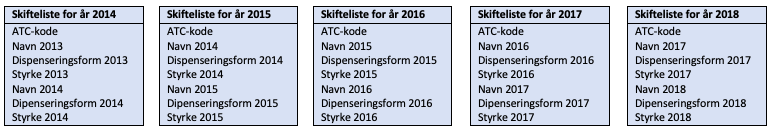
\includegraphics[width=1\textwidth]{billeder/Input1.png} 
	\caption{Skiftelister for år 2014, 2015, 2016, 2017 og 2018, indeholdende oplysninger om ATC-kode, lægemidlets navn, dispenseringsform og styrke.}
	\label{fig:Input}  
\end{figure}

Skiftelisterne kombineres med udbudsmateriale, der er udtrukket fra sygehusapoteksportalen, og indeholder oplysninger om blandt andet ATC-kode, lægemidlets navn, styrke og dispenseringsform samt priser og hvorvidt lægemidlet indgår i Medicinrådets behandlingsvejledning for de udbud som er gældende for det kommende år, hvilket fremgår af Figur \ref{fig:Input2}.
Indgår et lægemiddel i Medicinrådets behandlingsvejledning er det lovmæssigt bestemt, at disse skal anvendes som standardbehandling~\citep{Medicinradet2018}.
Ligeledes kombineres skiftelisterne med viden omkring kritiske ATC-koder og risikolægemidler. ATC-koder er indsamlet af SRN i forbindelse med problemstillinger vedrørende læggemiddelskift og omfatter ATC-koderne, som fremgår af Figur \ref{fig:Input2}. Risikolægemidler er indsamlet af Amgros og indeholder oplysninger om ATC-koder og lægemidlets navn. Disse lægemidler kan kræve et ekstra personalemæssigt ressourcetræk i forbindelse med lægemiddelskift, være forbundet med øget risiko for utilsigtede hændelser og/eller kritiske hvis de ender i restordre på grund af f.eks. leveringssvigt~\citep{Amgros}. 

\vspace{0.2cm}
\begin{figure}[H]\centering
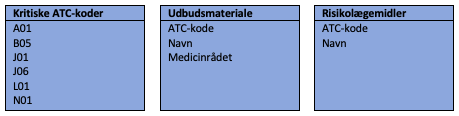
\includegraphics[width=0.6\textwidth]{billeder/Input2.png} 
	\caption{Udbudsmateriale, kritiske ATC-koder og risikolægemidler, der kombineres med skiftelister på baggrund af ATC-kode eller lægemidlets navn.}
	\label{fig:Input2}  
\end{figure}

\section{Risikofaktorer og vægtning}
Risikofaktorer er udvalgt ud fra den nuværende vurdering af medarbejdere, som er beskrevet af Afsnit \ref{sec:ImpLaeg}. Videnskabelig litteratur som beskriver risikofaktorer ved lægemiddelskift, der har ledt til medicineringsfejl i klinikken, hvilket er beskrevet af Afsnit \ref{sec:ProblemLaeg}. Dokumenterede ATC-koder af SRN, som har ledt til problemstillinger vedrørende lægemiddelskift og derfor anses som kritiske~\citep{SRN}. Risikolægemidler, der overvåges særligt af Amgros, som f.eks. er kritiske hvis de ender i restordre \citep{Amgros}. Risikofaktorerne er vægtet af en ekspert inden for området, hvoraf en vægtning på 1 anses som værende af mindre betydning for implementering af lægemiddelskift og derfor kræver mindre opmærksomhed. Derimod anses en vægtning på 5 som værende af stor betydning og kræver mere opmærksomhed ved implementering i klinikken.
Risikofaktorer og deres vægt samt begrundelse for valg fremgår af Tabel \ref{table:features}.


\begin{longtable}{|l|c|p{9.2cm}|}
	\caption{Risikofaktorer som anvendes i den nuværende vurdering af lægemiddelskift og er beskrevet i videnskabelig litteratur. Vægtningen af risikofaktorerne er foretaget af en ekspert inden for området, hvor en vægtning på 1 har mindre betydning, mens en vægtning på 5 har stor betydning ved implementeringen af lægemiddelskift.} 
	\label{table:features} \\ \hline
\cellcolor[HTML]{C0C0C0} {\textbf{Risikofaktor}} & \cellcolor[HTML]{C0C0C0} {\textbf{Vægt}} & \cellcolor[HTML]{C0C0C0} {\textbf{Begrundelse}} \vspace{0.2cm} \\ \hline
\textbf{Navn} & \textbf{1} & Dispensering af forkert lægemiddel sker typisk i forbindelse med forveksling af lægemiddelnavne~\citep{DanskSelskabforPatientsikkerhed2009}, hvilket kan give anledning til uønskede bivirkninger~\citep{Basco2010} og i sjældnere tilfælde forlænget indlæggelse, forværret sygdom eller dødsfald~\citep{DanskSelskabforPatientsikkerhed2009}.  \\  \hline 
\textbf{Look-a-likes} & \textbf{2} & En af de hyppigste årsager til dispensering af forkert lægemiddel er lignende navn~\citep{Hakonsen2010}. Look-a-likes har påvist, at kunne prædisponeres til medicineringsfejl~\citep{Wittich2014} og sandsynligheden for fejl ved look-a-like stiger med antallet af ortografiske ligheder~\citep{Basco2010}. \\  \hline 
\textbf{Dispenseringsform} & \textbf{2} & Dispensering af det forkerte lægemiddel, grundet navneforveksling, kan give anledning til fejl i dispenseringsform~\citep{DanskSelskabforPatientsikkerhed2009, Agrawal2009}, hvilket har betydning for virkningen af lægemidlet samt arbejdsgangen for sygehuspersonalet i forhold til brug af ekstra ressourcer og information.
\\ \hline 
\textbf{Styrke} & \textbf{2} & Styrke kan medføre medicineringsfejl ved ordination ved forkert styrkeberegning~\citep{Agrawal2009}, hvorfor der skal være opmærksom på ændringen i styrke for at undgå beregningsfejl, som kan medføre overdosering eller underdosering og derved påvirke patienten.\\ \hline
\textbf{Risikolægemidler} & \textbf{3} & Disse lægemidler overvåges særligt af Amgros, da de er kritiske ved restordre~\citep{Amgros}, kræver et ekstra personalemæssigt ressourcetræk i forbindelse med skift og er i øget risiko for utilsigtede hændelser~\citep{Amgros}. \\ \hline 
\textbf{ATC-grupper} & \textbf{5} & ATC-grupper som, A01, B05, J01, J06, L01 og N01 har givet anledning til problemstillinger vedrørende lægemiddelskift og kan derfor anses som kritiske\citep{SRN}. \\ \hline 
\textbf{Medicinråd} & \textbf{5} & Lægemidler, som indgår i Medicinrådets behandlingsvejledninger, er besluttet af Medicinrådet at skulle anvendes som standardbehandling~\citep{Medicinradet2018}. Disse vurderes i forhold til effekt, eksisterende behandling og pris~\citep{Medicinradet2018}. For disse lægemidler er der ofte mange besparelser at opnå ved hurtig og effektiv implementering.\\ \hline 
    \end{longtable}

\section{Præprocessering}
Præprocessering af data er foretaget, da data er tekstbaseret og indskrevet manuelt og derfor ikke sammenligneligt. Det er forskelligt om data er skrevet med majuskel eller minuskel, hvorfor det er valgt at ændre alt data til minuskel. Ligeledes er forkortelser udskrevet og tegnsætning fjernet for at gøre data generaliserbart. 
Synonymer, såsom filmovertrukne tabletter eller overtrukne tabletter, er fjernet og angivet som tabletter. 
Det varierer for styrke om der anvendes mellemrum mellem tal og enheder, hvorfor mellemrum er fjernet. 

Det er antaget for tomme tekstfelter at intet er ændret, hvormed data fra enten tidligere år eller for det kommende skift er gældende. For lægemidlets navn er det antaget at dette er ens, hvis præfiks er uændret, hvorfor suffiks er fjernet. Lægemidler med ens præfiks, men forskellig suffiks, kan give anledning til forskellige dispenseringsformer eller styrker. Hvis dette er tilfældet vil dette opdages i forbindelse med sammenligning af dispenseringsform og styrke. 

\section{Design}
%\textcolor{red}{Tilføj: Hvilke overvejelser har jeg gjort i design i forhold til at gøre systemet generealiserbart?} \\
Risikovurderingen er designet som if-then-else statements, der danner grundlag for risikovurderingen. For hvert statement vurderes én eller flere risikofaktorer i forhold til om et statement er sandt eller falsk. Ud fra antallet af sande statements beregnes risikoscoren ud fra Ligning \ref{equ:risikoscore} på baggrund af den totale vægt af matchende risikofaktorer og den totale vægt af alle risikofaktorer.

\begin{equation}  \label{equ:risikoscore}
Riskoscore = \frac{\mbox{\textit{Totale vægt af matchende risikofaktorer}}}{\mbox{\textit{Totale vægt af alle risikofaktorer}}} \cdot 100
\end{equation}

Risikoscoren er angivet som en procentdel, hvorved der er et bedre beslutningsgrundlag for at vurdere betydningen af risikoscoren. En høj risikoscore vil betyde at risikofaktorer, som gør sig gældende for lægemiddelskiftet gør implementeringen mere kompleks. Hvis risikoscoren modsat er lille vil lægemiddelskiftet være mindre kompleks at implementere. På denne måde kan medarbejderne fra SRN skelne mellem, hvilke lægemiddelskift der kræver ekstra opmærksomme og derfor kræver uddybende information til klinikken ved udarbejdelsen af Lægemiddel Nyt.  

Til design af look-a-likes lægemidler, der sammenligner hvorvidt et lægemiddels navn for det kommende skifteår ligner et andet lægemiddel, registreret ved tidligere lægemiddelskift, beregnes Levenshtein Distance. Levenshtein Distance er et udtryk for det minimale antal af operationer, der kræves for at ændre et ord til et andet ved at slette, indføre eller erstatte bogstaver~\citep{Schepens2012}. For at sikre at lægemidler er forholdsvis sammenlignelige fastsættes en grænse på maksimal fire antal operationer. Levenshtein Distancen beregnes ud fra Ligning \ref{equ:LevDistance} på baggrund af det minimale antal af tilføjede, slettede og erstattede bogstaver der kræves for at ændre et ord til et andet samt den maksimale længde af de to ord som sammenlignes. 

\begin{equation} \label{equ:LevDistance}
\mbox{\textit{Levenshtein Distance}} = 1 - \frac{\mbox{\textit{min(antal af tilføjede, slettede og erstattede bogstaver)}}}{\mbox{\textit{max(længde af ord der sammenlignes)}}}   
\end{equation}

Outputtet er designet ud fra, hvordan den nuværende vurdering af lægemiddelskift foregår. Da skiftelisterne er udarbejdet i excel-filer og medarbejderne er velkendt med dette layout er det valgt, at outputtet visualiseres i allerede eksisterende excel-filer. Udover de nuværende data tilføjes en ekstra kolonne til excel-filen, som indeholder risikoscore og begrundelse for denne. Designet af outputtet fremgår af Figur \ref{fig:Output}.

\vspace{0.2cm}
\begin{figure}[H]\centering
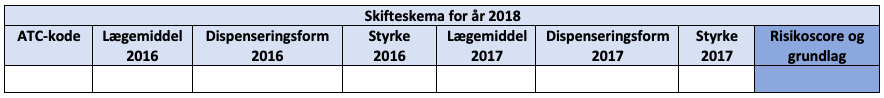
\includegraphics[width=1\textwidth]{billeder/Output.png} 
	\caption{Design af output. De lyseblå kasser symboliserer allerede eksisterende kolonner, hvor den mørkeblå kasse er tilføjet og indeholder output fra systemet, herunder risikoscore og begrundelse for denne.}
	\label{fig:Output}  
\end{figure}

\section{Implementering}
Systemet er implementeret i NetBeans, som er et Integrated Development Environment (IDE) til Java.  Java Excel API og Apache POI er tilføjet til biblioteket for at kunne indlæse og skrive i Microsoft dokumenter. For at kunne håndtere bogstaverne æ, ø og å er tegnsættet ændret til ISO-8859-15 i NetBeans IDE. Implementering af risikovurdering af lægemiddelskift fremgår af Appendiks \ref{App:Risikovurdering} og Levenshtein Distancen for sammenligning af look-a-likes fremgår af Appendiks \ref{App:LevDistance}.

\section{Evaluering}
Systemets anvendelighed er evalueret af medarbejdere fra SRN, som har erfaring med lægemiddelskift. Dette er gjort ved at evaluere systemet i forhold til risikoscore og begrundelse for denne, rangering af en række lægemiddelskift ud fra risikoscoren samt diskussion af risikofaktorer og vægtningen af disse. En introduktion til systemet blev givet inden evalueringen for at sikre en fælles forståelse for systemets risikovurdering af lægemiddelskift, denne fremgår af Appendiks \ref{App:Intro}. 

For at evaluere risikoscoren er 33 lægemiddelskift fra henholdsvis skift i år 2016, 2017 og 2018 vurderet med henblik på at undersøge, hvornår et lægemiddelskift kræver uddybende information inden implementering i klinikken. Disse er udvalgt på baggrund af risikoscoren og begrundelsen for denne i forhold til at repræsentere forskellige lægemiddelskift, som fremgår af Appendiks~\ref{App:Evaluering}. Ligeledes er rangeringen af lægemiddelskiftet vurderet samt risikofaktorer og deres vægtning diskuteret. 

Risikoscore og rangeringen af denne er sammenholdt med medarbejdernes vurdering og Lægemiddel Nyt for at undersøge overensstemmelse mellem disse. Ligeledes er sensitivitet og specificitet af risikoscoren udregnet i SPSS for at teste systemets nøjagtighed i forhold til at forudsige om et lægemiddelskift kræver uddybende information. Sammenhængen mellem sensitivitet og specificitet visualiseres af en Receiver Operating Characteristic (ROC) kurve, hvorefter nøjagtigheden af systemet opsummeres ved at beregne arealet under kurven. Ud fra ROC-kurven undersøges grænseværdier i forhold til at inddele lægemiddelskift ud fra risikoscoren for at identificere en grænse for, hvornår et lægemiddelskift kræver uddybende information.



